%%%% CAPÍTULO 3 - MATERIAL E MÉTODOS (PODE SER OUTRO TÍTULO DE ACORDO COM O TRABALHO REALIZADO)
%%
%% Deve apresentar o modelo utilizado, a modelagem
%% empregada, as simplificações necessárias, a
%% metodologia e a descrição do método de cálculo 
%% utilizado no desenvolvimento da pesquisa para que
%% a mesma possa ser reconstituída. Deve ainda 
%% apresentar resultados de amostras e comentários.
%% Deve apresentar a descrição da montagem 
%% experimental, metodologia para a obtenção de 
%% resultados, análise de erros, amostra de resultados
%% obtidos e comentários. Atenção: Esta parte pode ser
%% subdividida em mais capítulos de acordo com a 
%% especificidade do assunto.

%% Título e rótulo de capítulo (rótulos não devem conter caracteres especiais, acentuados ou cedilha)
\chapter{Software}\label{cap:materialemetodos}

\section{StateChart}

Nesta etapa de desenvolvimento, apresentamos o state chart do sistema embarcado desenvolvido para o scanner 3D, uma ferramenta crucial para a visualização e compreensão do comportamento dinâmico do sistema. O state chart é fundamental para garantir a precisão e eficiência do scanner, pois detalha os estados operacionais e as transições baseadas em eventos, permitindo uma implementação de software robusta e confiável. Através do diagrama da Figura \ref{foto:state} , é possível antecipar e resolver potenciais problemas, otimizando o processo de desenvolvimento e contribuindo significativamente para o sucesso do projeto.

\begin{figure}[H]
\captionsetup{width=0.6\textwidth}%% Largura da legenda
\caption{Statechart do Scanner 3D}%% Legenda
\label{foto:state}%% Rótulo
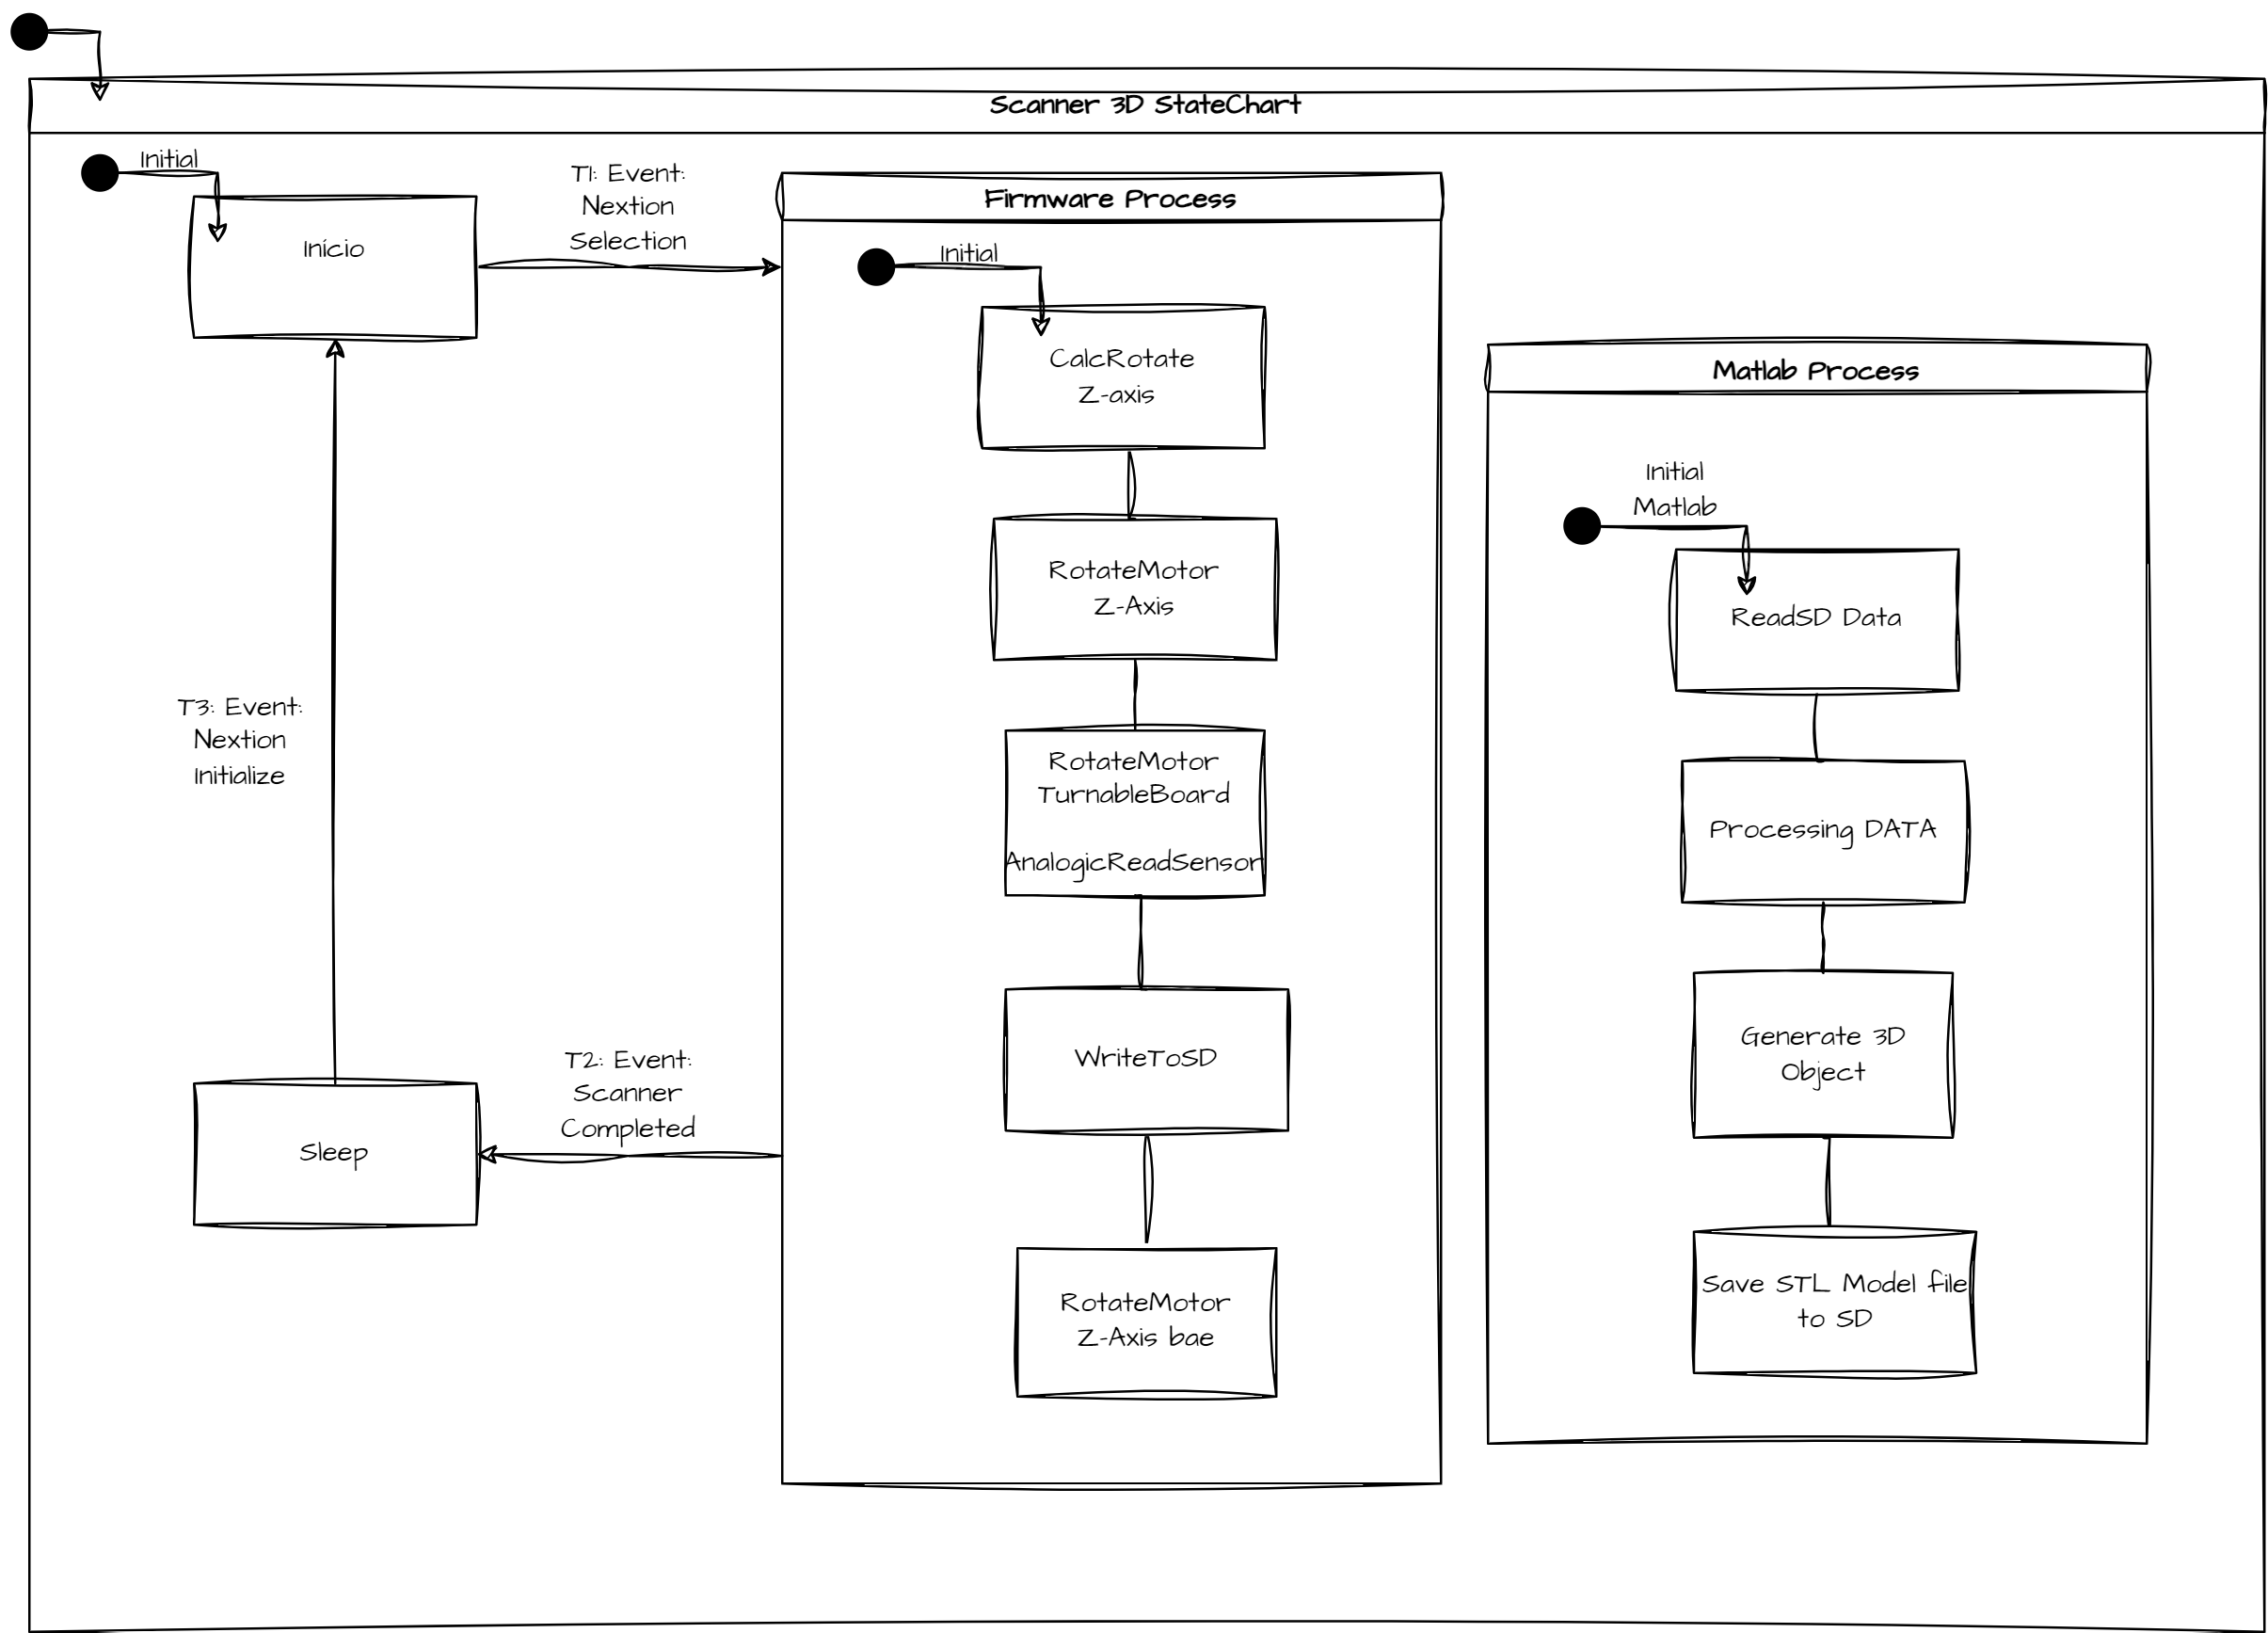
\includegraphics[width=\textwidth]{4.Software/Imagens/StateChartScanner3D.png}%% Dimensões e localização
\fonte{AUTORES}%% Fonte
\end{figure}


\section{Firmware}

\subsection{Ferramentas de Desenvolvimento}
O código fonte foi desenvolvido através do \textit{Visual Studio Code (VS Code)} \cite{site:vscode} por possuir uma estrutura que facilita a criação de arquivos e detecção de erros de sintaxe. Para a compilação do código e testes, foi utilizado o software \textit{Arduino IDE} \cite{site:arduino}, pois o código fonte utiliza bibliotecas que estão diretamente associadas ao arduino. O versionamento do código foi controlado através do repositório no \textit{GitHub} \cite{site:reposit_git}, este qual está disponível e pode ser visualizado de maneira pública.

\subsection{Software}

O fluxo geral apresentado na Figura  \ref{foto:fluxogeral} descreve o processo de operação de um sistema embarcado para um scanner 3D. Inicia-se com a configuração das variáveis e segue para a medição da distância vertical. Dependendo do resultado, o sistema pode ajustar a posição vertical ou prosseguir para a rotação do motor. O processo inclui etapas de decisão que determinam a direção e a quantidade de passos do motor, bem como a coleta de dados de distância e a gravação desses dados. O fluxo é iterativo e continua até que todas as condições necessárias sejam atendidas para completar a digitalização tridimensional do objeto. Este fluxo assegura a precisão e a eficiência na captura dos dados necessários para a modelagem 3D.

\begin{figure}[H]
\captionsetup{width=0.6\textwidth}%% Largura da legenda
\caption{Fluxograma Geral do Software}%% Legenda
\label{foto:fluxogeral}%% Rótulo
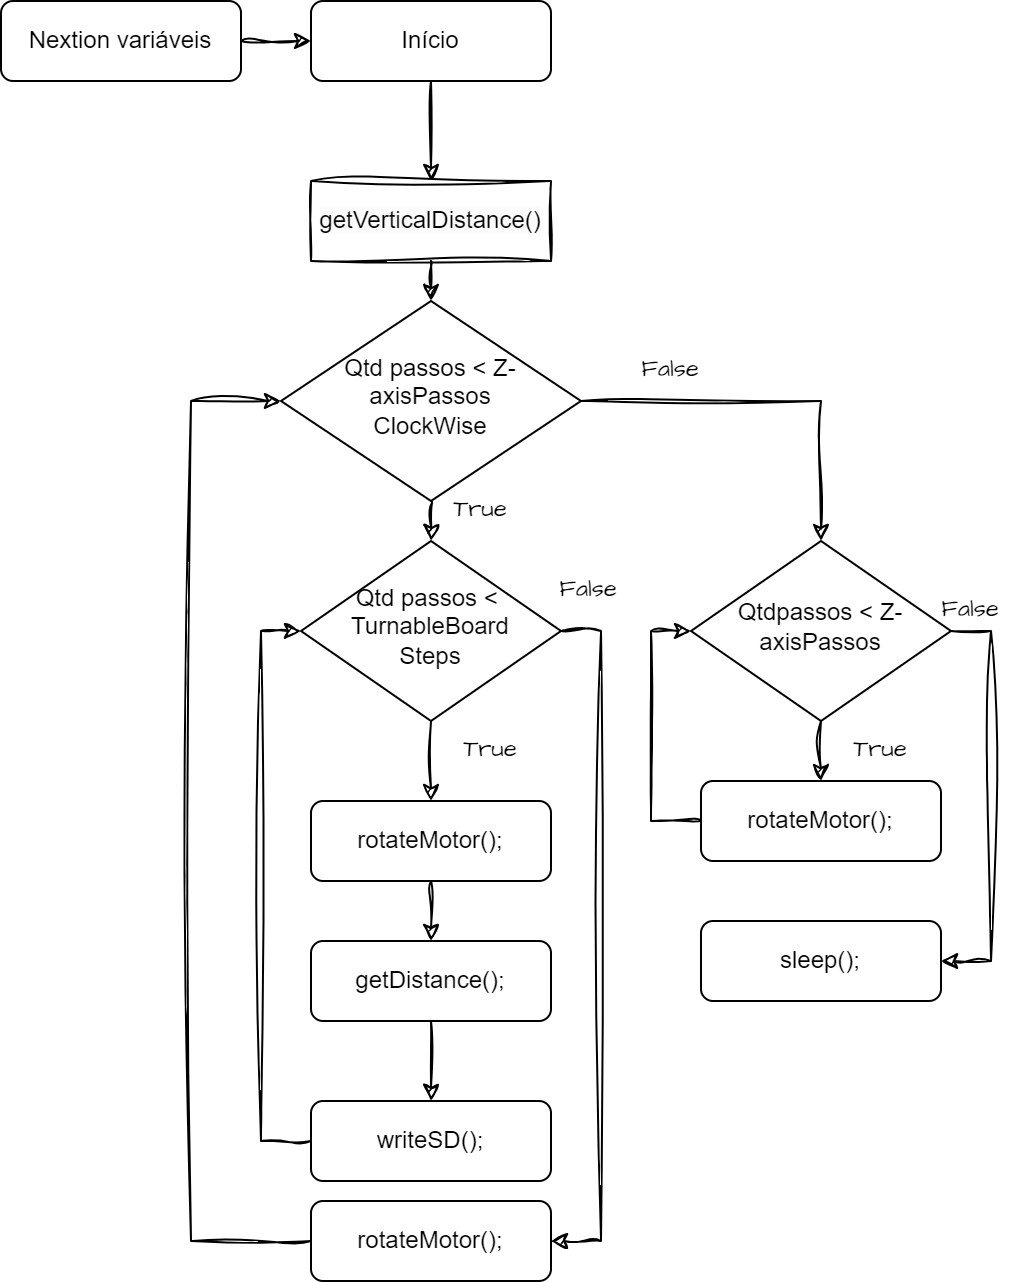
\includegraphics[width=\textwidth]{4.Software/Imagens/FluxoGeral.png}%% Dimensões e localização
\fonte{AUTORES}%% Fonte
\end{figure}

Na função principal do software, o sistema fica ocioso até receber o comando via Nextion. Basicamente, temos um loop principal responsável por controlar um processo de varredura (scan) de um objeto. A ideia principal desse processo é definir uma resolução de rotação dos motores de passo para captura dos pontos, seguido de uma detecção do comprimento do objeto scanneado, uma vez cumprido esse fluxo, temos um laço responsável pelo controle do motor da plataforma do sensor aninhado com o loop de rotação da plataforma giratória onde o objeto se encontra. Terminada a etapa de captura, a variável de controle do eixo Z-axis, comanda o laço que retorna a plataforma do sensor naturalmente para sua posição de origem, o que ocasiona o fim do objetivo do sistema. 


\subsubsection{Fluxogramas das funções desenvolvidas}

Como exposto na Figura \ref{foto:rotate}, a função é projetada para controlar a rotação de um motor de passo conectado ao pino especificado, isto é, o pino proveniente da plataforma do sensor ou da mesa giratória. Ela permite especificar o número de passos que o motor deve girar, o que pode ser usado para controlar a posição ou o movimento de um dispositivo.

\begin{figure}[H]
\captionsetup{width=0.6\textwidth}%% Largura da legenda
\caption{Fluxograma: função void rotateMotor(int pinNo, int steps);}%% Legenda
\label{foto:rotate}%% Rótulo
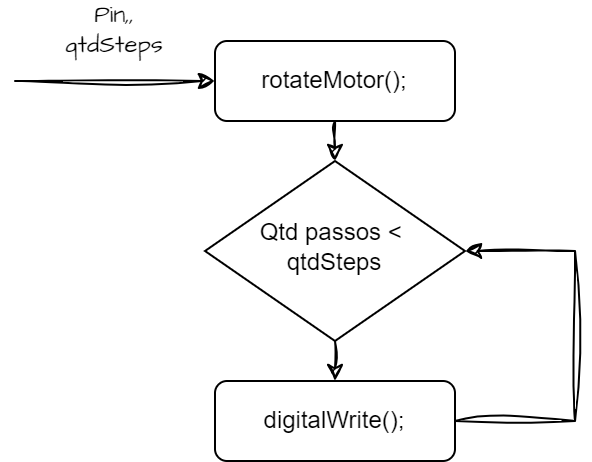
\includegraphics[width=\textwidth]{4.Software/Imagens/Rotate.png}%% Dimensões e localização
\fonte{AUTORES}%% Fonte
\end{figure}

De acordo com a Figura  \ref{foto:getVertical}, a função controla o motor responsável por elevar e abaixar o sensor infravermelho, capturando a distância vertical de um objeto colocado na base giratória. A função realiza sua medição em passos, subindo até o sensor não mais detectá-lo (indicando que atingiu o topo), e depois retornando à posição inicial. A condição de detecção é baseada em valores negativos do sensor, indicando que nada está no seu alcance de captura.

\begin{figure}[H]
\centering
\captionsetup{width=0.6\textwidth} % Set the width of the caption
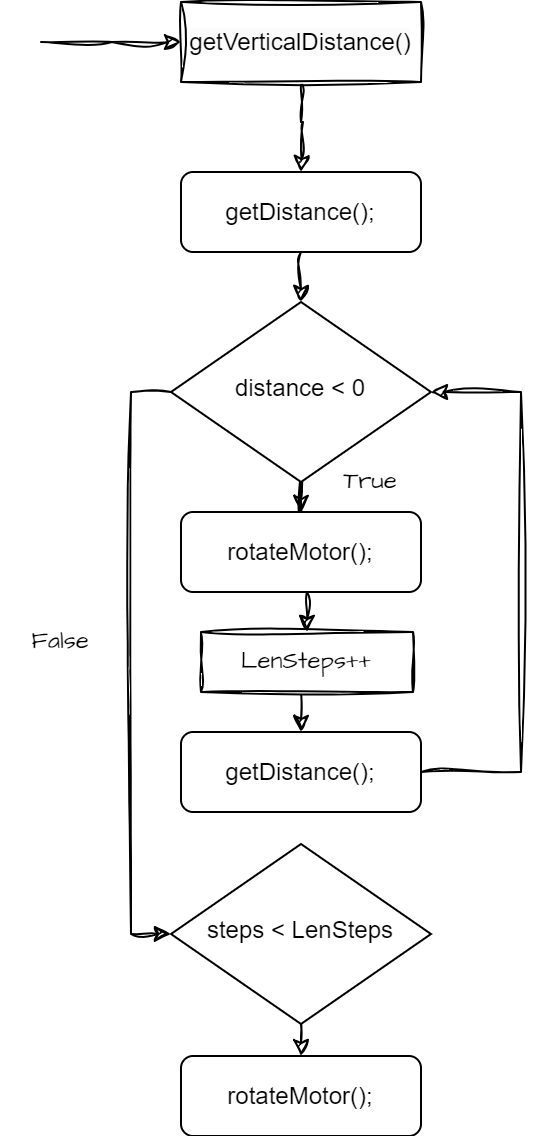
\includegraphics[width=0.5\textwidth]{4.Software/Imagens/getVerticalDistance.png} % Adjust the width of the image
\caption{Fluxograma: função int getVerticalDistance();}
\label{foto:getVertical}
\fonte{AUTORES}
\end{figure}

Por último, temos a função mais importante do sistema. Como exemplificado na Figura \ref{foto:getDistance}, ela é é projetada para medir a distância do sensor até o objeto e, em seguida, calcular as coordenadas \textbf{(x, y)} com base na distância e no ângulo capturado no ponto do objeto para uma variação em radianos dos passos da base giratória.
A função que realiza a leitura analógica e a média inicia um loop para ler valores de um sensor analógico múltiplas vezes, acumulando essas leituras e calculando a média para obter um valor mais estável e menos suscetível a ruídos. Em seguida, o valor médio é convertido de uma leitura analógica (variando de 0 a 1023) para uma tensão (de 0 a 5V) usando a função mapDouble. Essa conversão é necessária porque a calibração do sensor é fornecida em termos de tensão.

A tensão obtida é então convertida para uma distância em centímetros utilizando uma fórmula cúbica derivada da calibração do sensor, baseada em dados do datasheet do sensor específico utilizado. Após o cálculo da distância, um ajuste é realizado subtraindo essa distância de uma distância fixa, que representa a distância do sensor até um ponto de referência central. Esse ajuste é feito para obter a distância real do objeto até o ponto de referência.

Finalmente, as coordenadas (x, y) são calculadas utilizando funções trigonométricas (cos e sin) do ângulo do sensor e da distância ajustada. Esse processo permite mapear a posição do objeto em um plano 2D em relação ao ponto de referência. Além disso, a coordenada Z advém da plataforma do sensor, assumindo inicialmente o valor 0 e sendo incrementada de acordo com o número de steps do motor que eleva o sensor verticalmente. Assim, conforme o sensor se move para cima, a coordenada Z é ajustada para refletir a nova posição vertical do sensor. A função não retorna um valor diretamente, e os resultados do cálculo (distância e coordenadas x e y) são armazenados em variáveis globais e posteriormente passados para a memória SD.

\begin{figure}[H]
\captionsetup{width=0.6\textwidth}%% Largura da legenda
\caption{Fluxograma: função void getDistance();}%% Legenda
\label{foto:getDistance}%% Rótulo
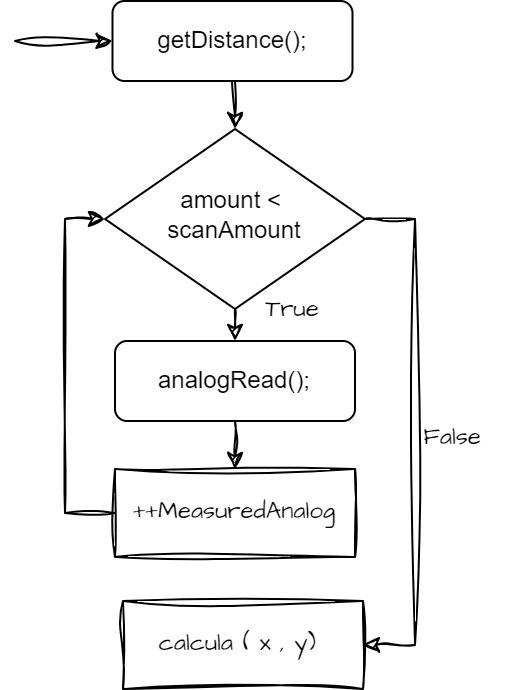
\includegraphics[width=\textwidth]{4.Software/Imagens/getDistance.png}%% Dimensões e localização
\fonte{AUTORES}%% Fonte
\end{figure}

\subsection{Interface}

A interface de usuário do projeto de Scan 3D foi projetada para ser simples e intuitiva, facilitando a operação do dispositivo por qualquer usuário, independentemente de seu nível de experiência técnica. A interface consiste em dois botões principais: "Start" e "Stop", e é implementada via display Nextion.

O botão "Start" é utilizado para iniciar o processo de escaneamento. Quando pressionado, ele ativa o programa que controla o scanner 3D. O dispositivo começa a capturar as coordenadas tridimensionais do objeto colocado na base giratória. O sensor infravermelho se movimenta verticalmente ao longo do eixo Z, enquanto a base giratória, controlada por um motor de passo, roda o objeto para que todas as suas dimensões sejam mapeadas com precisão. Durante este processo, os dados de distância são coletados e armazenados.

O botão "Stop" serve para interromper o processo de escaneamento e reiniciar o programa. Quando pressionado, ele não apenas para a captura de dados, mas também retorna o eixo Z do motor para a posição inicial. Este recurso é crucial para garantir que o scanner esteja pronto para um novo ciclo de escaneamento sem a necessidade de ajustes manuais, proporcionando conveniência e economia de tempo para o usuário.

Após a conclusão da captura, os dados são transferidos para um cartão SD e posteriormente processados no software Matlab para gerar um modelo digital detalhado do objeto. A simplicidade desta interface, com apenas dois botões, garante que o foco do usuário permaneça no processo de digitalização do objeto, sem a necessidade de navegar por menus complexos ou realizar configurações adicionais.

